\documentclass[letterpaper,11pt]{article}

\usepackage{geometry, pslatex, fancyhdr, graphicx}
\usepackage{amsmath,amsthm,amssymb,scrextend}
\usepackage{multicol}
\usepackage{tabularx}
\usepackage[makeroom]{cancel}
\usepackage{color}
\usepackage{tabto}
\geometry{ margin = 1.0in }

%%% TODO modify these variables as per your homework %%%
\def\homeworknum{3}
\def\myname{Harshit Jain}
\def\myuserid{hmj5262}
%%%%

\pagestyle{fancy}
\lhead{{\bf CMPSC 461 Spring 2023}}
\chead{{\bf Assignment~\homeworknum}}
\rhead{{\bf \today}}
\let\newproof\proof
\renewenvironment{proof}{\begin{addmargin}[1em]{0em}\begin{newproof}}{\end{newproof}\end{addmargin}\qed}

\newcounter{problemid}
\stepcounter{problemid}
\def\newproblem{\clearpage\newpage{\bf Problem~\arabic{problemid}\stepcounter{problemid}}\hfill\par}

\setlength\parindent{0em} 
\setlength\parskip{8pt}
\setlength{\fboxsep}{6pt}


\begin{document}

\framebox[\textwidth]{
	\parbox{0.96\textwidth}{
		\parbox{0.12\textwidth}{\bf Name:}\parbox{0.6\textwidth}{\myname}\\
		\parbox{0.12\textwidth}{\bf User ID:}\parbox{0.6\textwidth}{\myuserid}
	}
}
%% your solutions %%%


% PROBLEM 1
\newproblem 
\begin{enumerate}
    
    \item
    $35$ $26$ $25$
    
    $5$ $10$ $15$
    
    \item 
    
    $35$ $26$ $15$

    $35$ $26$ $15$
    
    \item 
    
    $35$ $26$ $25$
    
    $5$ $10$ $15$
    
    \item 
    
    $55$ $26$ $25$
    
    $5$ $10$ $15$

\end{enumerate}


% PROBLEM 2
\newproblem 
\begin{enumerate}
    
    \item
    $10$ $39$ $25$
    
    $10$ $15$
    
    \item 
    
    $44$ $44$ $25$

    $44$ $15$
    
    \item 
    
    $10$ $39$ $25$
    
    $39$ $15$
    
    \item 
    
    $49$ $49$ $64$
    
    $49$ $15$ 
     
\end{enumerate}


% PROBLEM 3
\newproblem 
\begin{enumerate}

    \item False. Maintenance of the subroutine call stack is the responsibility of the callee.
    Explanation: The callee is responsible for saving and restoring the caller's context, including the return address and any callee-saved registers, on the stack before executing the subroutine.
    
    \item True. Modern machines typically pass subroutine parameters in stacks.
    Explanation: In most modern machines, subroutine parameters are passed in a stack-based calling convention.
    
    \item False. Subroutine calling convention gives the callee the responsibility to save all the registers that it modifies.
    Explanation: The callee is responsible for saving and restoring any registers that it modifies during the subroutine call, but the caller is responsible for saving and restoring any registers that it needs to preserve across the call.
    
    \item True. Parameter-passing in C is call-by-value as well as call-by-reference (when using pointers).
    Explanation: In C, function parameters are passed by value by default, but it is possible to pass a pointer to a variable and modify the value indirectly, effectively passing it by reference.
    
    \item False. The calling sequence convention used by a compiler is not specified by the language and can vary depending on the platform and the optimization level.
    Explanation: The calling sequence convention used by a compiler is not part of the language specification and can vary depending on the platform and the optimization level.
    
    \item True. It is the caller's responsibility to maintain the static chain during a subroutine call.
    Explanation: The static chain is used to access variables in higher-level scopes, and it is the caller's responsibility to set up the static chain correctly before calling a subroutine.
    
    \item True. Pascal is call by value but can do call by reference with the help of the keyword 'var'.
    Explanation: In Pascal, function parameters are passed by value by default, but the 'var' keyword can be used to pass a parameter by reference.
    
    \item False. For C++ function header "void f1(int p1, float\& p2);", $p1$ is passed by value and $p2$ is passed by reference.
    Explanation: In the given function header, $p1$ is passed by value, and $p2$ is passed by reference.   
    
\end{enumerate} 


% PROBLEM 4
\newproblem
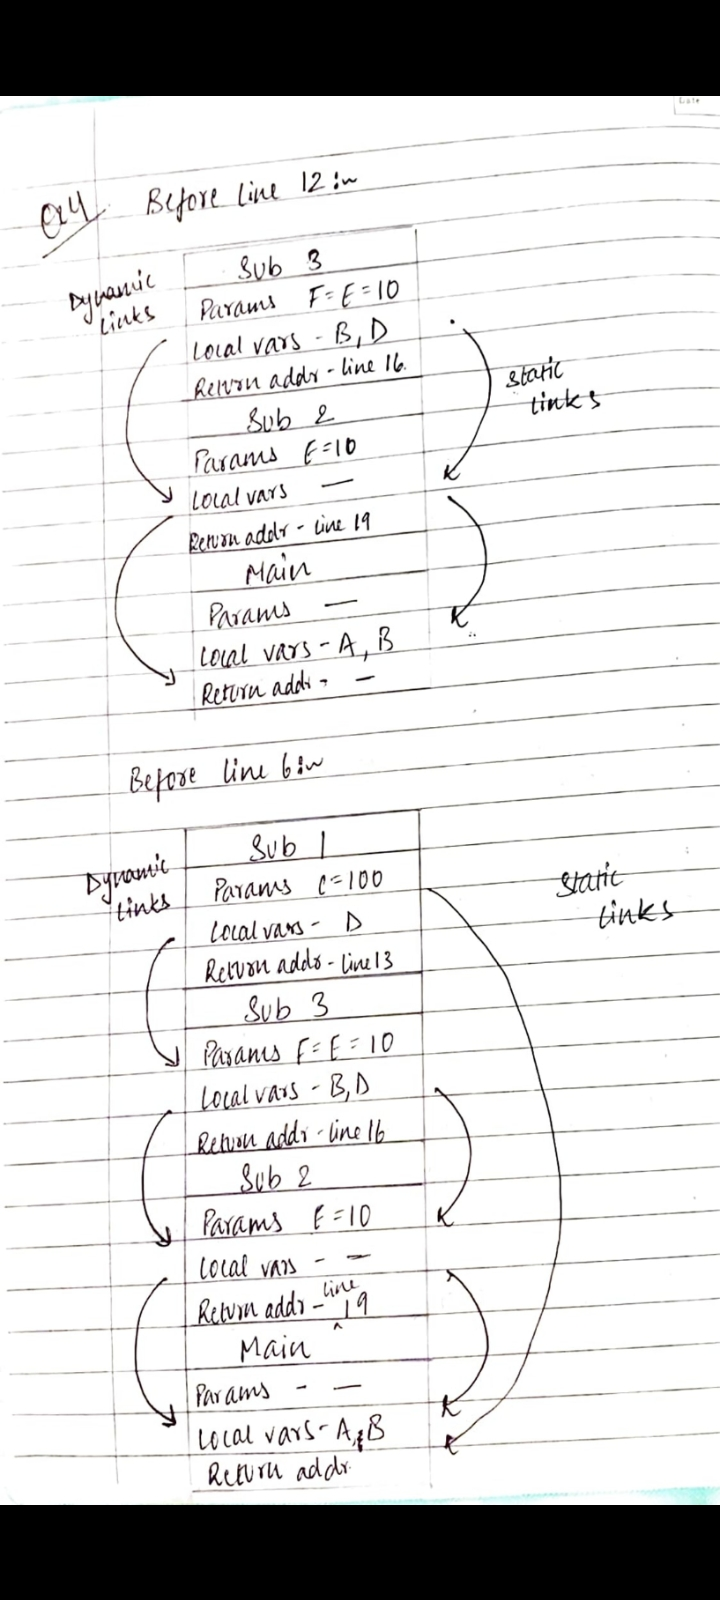
\includegraphics[scale = 0.35]{4}

% PROBLEM 5
\newproblem 
In call-by-sharing, also known as call-by-object-sharing, the function receives a reference to the object as a parameter, but the function does not receive the object itself. The object is still stored in the caller's memory, and any changes made to the object within the function are reflected in the caller's memory.

Call-by-sharing is similar to call-by-reference, but there is a subtle difference. In call-by-reference, the function receives a reference to the variable itself and any changes made to the variable within the function are reflected in the caller's memory. On the other hand, in call-by-sharing, the function receives a reference to the object, but not to the variable itself. Any changes made to the object within the function are reflected in the caller's memory, but if the function reassigns the reference to a new object, this change is not reflected in the caller's memory.

Call-by-value, on the other hand, passes a copy of the value of the variable to the function. Any changes made to the variable within the function are not reflected in the caller's memory.


% PROBLEM 6
\newproblem

\begin{enumerate}
    
    \item We should use Dynamic scoping as we want to swap the values in the caller. We would want the arguments to be evaluated in caller's environment.
    
    \item Yes, there will be problems while calling $exchange(s,t)$ as we are using pass-by-name. Line $5$ will become $t=t$ creating a confusion between a local variable and existing variable. To fix it, we should name the local variable.
    
    \item Yes, there will be a problem here. Since, parameter $'a'$ is being changed first, value of $i$ will change first. This will lead to some different index in array or index-out-of-bounds error. This leads to wrong implementation of function. To fix this problem, we can implement it in a following way: 
    
    function exchange(a,b)
    \tabto{20pt} var t = b
    \tabto{20pt} start
    \tabto{40pt} b = a
    \tabto{20pt} a = t
    \tabto{20pt} end
\end{enumerate}



\end{document}